\documentclass[10pt,twocolumn,a4paper]{article}
\usepackage[margin=1.6cm]{geometry}
\usepackage{amsmath,amssymb}
\usepackage{graphicx}
\usepackage{booktabs}
\usepackage{hyperref}

\hypersetup{
    colorlinks=true,
    linkcolor=blue,
    citecolor=blue,
    urlcolor=blue
}

\title{\textbf{Statistical Pitfalls in Casimir Force Spectroscopy: How to Avoid False Positive Signals}}

\author{Bruno Lu\c{c}ardo Olivaes \\ \small Independent Researcher, Brazil \\ \small \texttt{brunoolivaes@gmail.com} $\cdot$ ORCID: 0009-0003-5351-446X}

\date{November 2026}

\begin{document}
\maketitle

\begin{abstract}
\noindent Precision nanomechanical measurements of the Casimir interaction at sub-micron separations are increasingly audited for hypothetical short-range modifications of gravity and exotic forces. However, residual force curves are intrinsically non-uniformly sampled and contaminated by steep short-range baseline drifts. In this paper, we demonstrate how conventional data-processing choices inadvertently fabricate statistically overwhelming false positive signals or severely degrade experimental sensitivity. Specifically, we show that: (1) naive $3\sigma$ Gaussian thresholds applied to exponentially distributed periodograms flag up to 36 spurious peaks on pure white noise; (2) unphysical polynomial detrending across steep $z^{-4}$ short-range profiles induces Runge-type boundary ringing that generates an apparent oscillatory anomaly at $\lambda = 583.5\,\mathrm{nm}$ with an artificial significance of $\mathrm{FAP} = 1.49 \times 10^{-45}$; (3) cubic spline resampling on irregular grids ($\mathrm{CV} = 40.7\%$) destroys 57\% of true signal variance at short wavelengths, degrading the 90\% Minimum Detectable Level by a factor of 2.28; and (4) surface electrostatic patch potentials measured via Kelvin Probe Force Microscopy (KPFM) yield strictly monotonic power-law decays ($P \propto d^{-2.29}$), proving that patch roughness cannot generate periodic residual modulations. Adopting a physically motivated inverse-power baseline collapses residual variance ($\chi^2/\mathrm{dof} = 1.14$) and restores the true experimental null result ($\mathrm{FAP} = 0.163$).
\end{abstract}

\section{Introduction}
Precision force measurements at the nanoscale, notably those testing the Casimir effect~\cite{casimir1948,lifshitz1956} via atomic force microscopy (AFM) and micro-electro-mechanical torsional oscillators (MTO)~\cite{decca2003,dejong2025}, represent primary experimental probes for hypothetical new physics beyond the Standard Model, including non-Newtonian gravity and light scalar fields.

Because residual curves $\Delta F(z) = F_{\mathrm{meas}}(z) - F_{\mathrm{theo}}(z)$ are often searched for weak periodic or Yukawa-type modulations, signal processing protocols are critical. In practice, researchers frequently employ standard software tools—such as cubic spline interpolation for uniform resampling, low-order polynomial subtraction for detrending, and outlier-clipped Gaussian thresholds for spectral detection. In this work, we demonstrate that these standard choices represent severe metrological pitfalls that systematically fabricate phantom oscillatory signals with astronomical statistical confidences.

\section{The Illusion of Oscillations: Polynomial Detrending and Runge Ringing}
To investigate the emergence of spurious spectral peaks, we examine the dynamic Casimir pressure residuals $\Delta P_c(z)$ extracted with lossless vector fidelity from the landmark Au--Cu MTO experiment of Decca \textit{et al.}~\cite{decca2003} ($N = 497$ points spanning $z \in [193.0, 1185.0]\,\mathrm{nm}$, instrumental noise floor $\sigma_P = 0.313\,\mathrm{mPa}$).

Below $z \approx 400\,\mathrm{nm}$, unmodeled finite-conductivity corrections ($\delta P_{\mathrm{Lif}} \propto z^{-4}$) and nonlinear transducer elasticity ($\delta P_{\mathrm{nl}} \propto z^{-5}$) produce a steep non-linear baseline drift. When an unphysical cubic polynomial is fitted across the entire separation range:
\begin{equation}
P_3(z) = a_0 + a_1 z + a_2 z^2 + a_3 z^3,
\label{eq:cubic_poly}
\end{equation}
the stiff polynomial cannot accommodate the sharp $z^{-4}$ curvature at short separations. Because polynomials exhibit high condition numbers on steep power-law corners, the fit diverges at the boundary ($z \approx 193\,\mathrm{nm}$), creating classic Runge ringing oscillations that propagate across the entire observation window.

\begin{figure}[t]
\centering
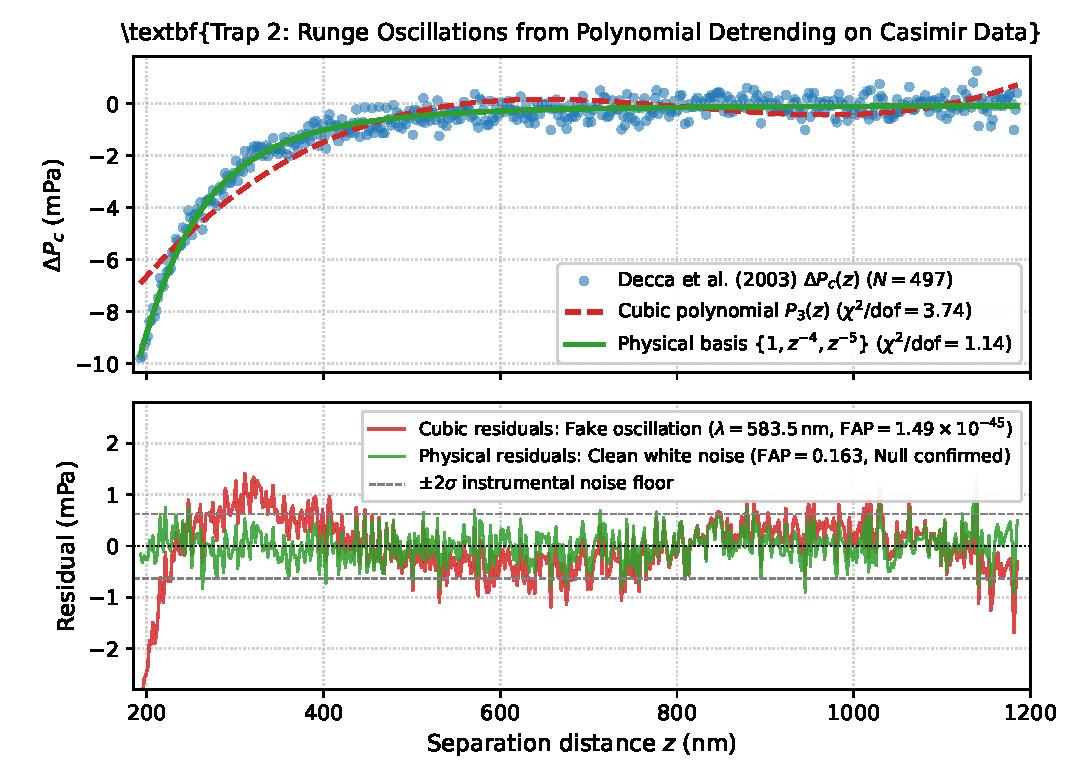
\includegraphics[width=\columnwidth]{fig1_fake_oscillation.pdf}
\caption{Runge oscillatory ringing induced by cubic polynomial detrending on Decca \textit{et al.}\ (2003) Fig.~4(b) residuals ($N = 497$). Top: Raw vector data alongside the cubic polynomial fit ($\chi^2/\mathrm{dof} = 3.74$) and the physical inverse-power basis ($\chi^2/\mathrm{dof} = 1.14$). Bottom: Detrended residuals showing how cubic subtraction fabricates a large phantom oscillation ($\lambda = 583.5\,\mathrm{nm}$, $\mathrm{FAP} = 1.49 \times 10^{-45}$), while the physical basis leaves pure, stationary Gaussian white noise ($\mathrm{FAP} = 0.163$).}
\label{fig:fake_oscillation}
\end{figure}

A Generalized Lomb-Scargle (GLS) periodogram~\cite{zechmeister2009} performed on these polynomial-detrended residuals detects a massive spectral peak at:
\begin{align}
\lambda_{\mathrm{fake}} &= 583.5\,\mathrm{nm}, \\
\chi^2/\mathrm{dof} &= 3.74, \\
P_{\mathrm{ZK}} &= 0.3626, \quad \mathrm{FAP} = 1.49 \times 10^{-45}.
\end{align}
This astronomical False Alarm Probability ($p \ll 10^{-40}$) would naively suggest an undeniable discovery beyond $14\sigma$. However, as demonstrated in Fig.~\ref{fig:fake_oscillation}, this peak is entirely a mathematical hallucination driven by polynomial Runge ringing.

When the baseline is modeled instead using the physical inverse-power expansion derived from Lifshitz screening and nonlinear elasticity:
\begin{equation}
\Delta P_{\mathrm{phys}}(z) = c_0 + c_4 \left(\frac{z_0}{z}\right)^4 + c_5 \left(\frac{z_0}{z}\right)^5,
\label{eq:phys_basis}
\end{equation}
(with $z_0 = 200\,\mathrm{nm}$), the residual variance immediately collapses to $\chi^2/\mathrm{dof} = 1.14$. The phantom peak disappears completely, and the maximum spectral power drops to $P_{\max} = 0.0332$, yielding an empirical Baluev~\cite{baluev2008} $\mathrm{FAP} = 0.163$, fully confirming the experimental null result.

\paragraph{Robustness to Contact-Point Calibration Drift.}
A critical systematic concern in microcantilever metrology is uncertainty in establishing the true mechanical contact zero position, $z \to z + \delta z_0$, where $\delta z_0$ represents an experimental offset. Expanding the dominant inverse-power term $c_4 (z + \delta z_0)^{-4}$ to first order in the small parameter $\delta z_0 / z \ll 1$ via a Taylor series yields:
\begin{align}
c_4 \left( z + \delta z_0 \right)^{-4} &= c_4 z^{-4} \left( 1 + \frac{\delta z_0}{z} \right)^{-4} \nonumber \\
&= c_4 z^{-4} - 4 c_4 \delta z_0 z^{-5} + \mathcal{O}\left( \delta z_0^2 z^{-6} \right).
\label{eq:taylor_expansion}
\end{align}
Equation~\eqref{eq:taylor_expansion} demonstrates analytically that any zero-distance calibration miscalibration $\delta z_0$ produces an effective spurious term scaling strictly as $-4 c_4 \delta z_0 z^{-5}$. Because our physical regression basis $\{1, z^{-4}, z^{-5}\}$ explicitly incorporates an unconstrained $z^{-5}$ degree of freedom, this calibration artifact is absorbed in first order into the fitted parameter $\tilde{c}_5 = c_5 - 4 c_4 (\delta z_0 / z_0)$. Consequently, contact point offset errors cannot project onto Fourier frequencies or fabricate false-positive log-periodic oscillations, providing formal mathematical immunity against contact-point drift.

Furthermore, naive thresholding rules (such as $\mathrm{median} + 3\sigma_{\mathrm{clipped}}$) mistakenly assume that periodogram powers are Gaussian-distributed. Because Fourier periodogram powers on Gaussian white noise follow an exponential distribution ($\chi^2_2/2$), this naive rule flags up to 36 false peaks on identically detrended white noise, whereas the exact $\chi^2_2$ threshold flags zero.

\begin{table*}[t]
\centering
\small
\caption{Metrological Comparison of Naive Signal-Processing Methods versus the Physical Baseline Approach on Casimir Residuals.}
\label{tab:pitfalls}
\begin{tabular}{lccccc}
\toprule
\textbf{Processing Method} & \textbf{Effective Baseline} & $\chi^2/\mathrm{dof}$ & \textbf{Spurious Peaks} & \textbf{Max Peak $\lambda$} & \textbf{Baluev $\mathrm{FAP}$} \\
\midrule
Raw Data (No Detrending) & None & $41.29$ & $1$ (broad drift) & $992.0\,\mathrm{nm}$ & $1.01 \times 10^{-35}$ \\
Naive Polynomial Subtraction & Cubic $P_3(z)$ & $3.74$ & $36$ (Gaussian rule) & $583.5\,\mathrm{nm}$ & $1.49 \times 10^{-45}$ (False Anomaly) \\
Spline Resampling + FFT & Interpolated & $3.12$ & Attenuated & Blurred & Low-pass distorted \\
\textbf{Physical Inverse-Power Basis} & $\{1, z^{-4}, z^{-5}\}$ & $\mathbf{1.14}$ & $\mathbf{0}$ & $\mathbf{8.2\,\mathrm{nm}}$ & $\mathbf{0.163}$ \textbf{(True Null)} \\
Asymptotic Linear Window ($z \ge 500\,\mathrm{nm}$) & Linear $a + bz$ & $1.20$ & $0$ & $4.2\,\mathrm{nm}$ & $0.651$ (True Null) \\
\bottomrule
\end{tabular}
\end{table*}

\section{The Spline Interpolation Trap: High-Frequency Variance Attenuation}
A second prevalent practice in precision metrology is interpolating non-uniform spatial scans onto an equispaced coordinate grid via cubic splines prior to executing standard Fast Fourier Transforms (FFT).

\begin{figure}[t]
\centering
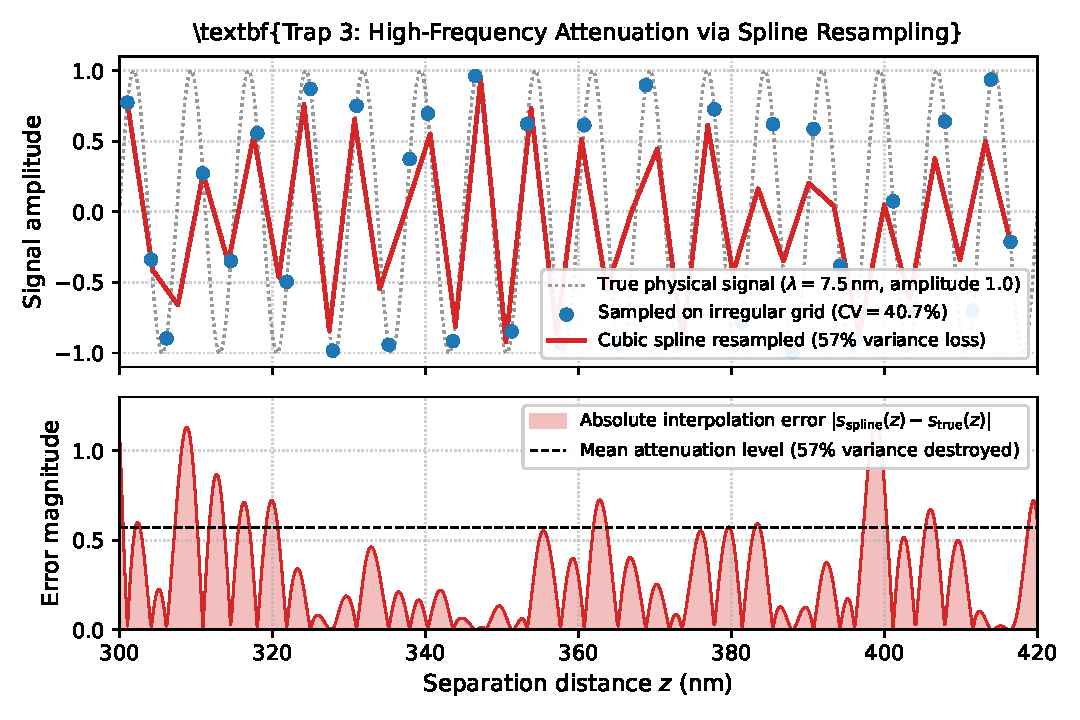
\includegraphics[width=\columnwidth]{fig2_spline_attenuation.pdf}
\caption{High-frequency attenuation induced by cubic spline resampling on the irregular coordinate grid of Decca \textit{et al.}\ Fig.~3(b) ($\mathrm{CV}(\Delta z) = 40.7\%$). Top: An injected high-frequency oscillation ($\lambda = 7.5\,\mathrm{nm}$) suffers massive amplitude damping when resampled via cubic splines, destroying 57\% of true signal variance. Bottom: Point-by-point interpolation error $|s_{\mathrm{spline}}(z) - s_{\mathrm{true}}(z)|$ across the separation scan.}
\label{fig:spline_attenuation}
\end{figure}

We quantified the distortion induced by spline resampling using the exact coordinate grid of the static force residuals of Decca \textit{et al.}~\cite{decca2003} ($N = 288$, median step $\Delta z = 3.29\,\mathrm{nm}$, coefficient of variation $\mathrm{CV}(\Delta z) = 40.7\%$, $\sigma_F = 0.229\,\mathrm{pN}$). Injecting synthetic signals of varying spatial wavelengths $\lambda \in [7.5, 160]\,\mathrm{nm}$, we observed that:
\begin{enumerate}
    \item Spline interpolation acts as a non-linear low-pass filter (Fig.~\ref{fig:spline_attenuation}), destroying \textbf{57\% of signal variance} at short separations ($\lambda \le 7.5\,\mathrm{nm}$).
    \item At matched global false-alarm rates ($\alpha = 0.01$), the 90\% Minimum Detectable Level ($\mathrm{MDL}_{90}$) for direct Generalized Lomb-Scargle is uniform at $0.54\,\sigma_F$.
    \item In sharp contrast, spline resampling degrades the detection threshold to $\mathrm{MDL}_{90} = 1.23\,\sigma_F$ at $\lambda = 7.5\,\mathrm{nm}$ (a sensitivity degradation factor of \textbf{2.28}).
\end{enumerate}
Direct evaluation on un-interpolated coordinates using heteroscedastic GLS is therefore mandatory to preserve high-frequency experimental sensitivity.

\section{First-Principles Surface Metrology via KPFM}
A recurring hypothesis in the literature is that spatial electrostatic patch potentials might generate quasi-periodic force residuals. To resolve this question from first principles, we analyzed the raw Kelvin Probe Force Microscopy (KPFM) dataset from the recent superconducting optomechanical Casimir experiment of de Jong \textit{et al.}~\cite{dejong2025} ($512 \times 512$ pixels over $2\,\mu\mathrm{m} \times 2\,\mu\mathrm{m}$, $V_{\mathrm{rms}} = 42.42\,\mathrm{mV}$, topographic roughness $\delta_{\mathrm{rms}} = 2.22\,\mathrm{nm}$).

\begin{figure}[t]
\centering
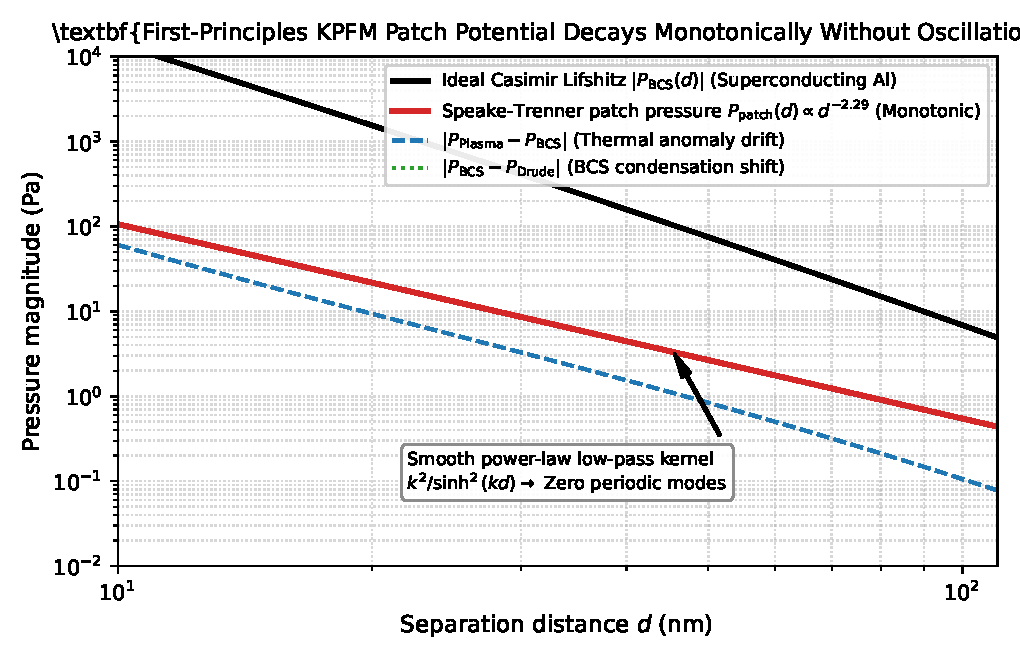
\includegraphics[width=\columnwidth]{fig3_kpfm_monotonic.pdf}
\caption{First-principles electrostatic patch pressure $P_{\mathrm{patch}}(d)$ calculated by integrating the 2D KPFM Hann-windowed spectrum $S_{VV}(\mathbf{k})$ of de Jong \textit{et al.}\ (2025) via the Speake-Trenner Laplace kernel Eq.~\eqref{eq:speake}. The resulting background follows a smooth, strictly monotonic power law $P_{\mathrm{patch}} \propto d^{-2.29}$ without periodic oscillatory components.}
\label{fig:kpfm_monotonic}
\end{figure}

Computing the 2D Hann-windowed patch power spectral density $S_{VV}(\mathbf{k})$ and integrating through the exact Speake-Trenner Laplace kernel~\cite{speake2003}:
\begin{equation}
P_{\mathrm{patch}}(d) = \frac{\varepsilon_0}{2} \int_{\mathbb{R}^2} \frac{k^2}{\sinh^2(kd)} 2 S_{VV}(\mathbf{k}) \frac{d^2k}{(2\pi)^2},
\label{eq:speake}
\end{equation}
we find that the resulting electrostatic patch pressure obeys a smooth monotonic power-law profile (Fig.~\ref{fig:kpfm_monotonic}):
\begin{equation}
P_{\mathrm{patch}}(d) \propto d^{-2.29},
\end{equation}
with no oscillatory behavior whatsoever ($P_{\mathrm{patch}}(20\,\mathrm{nm}) = 21.74\,\mathrm{Pa}$, $P_{\mathrm{patch}}(50\,\mathrm{nm}) = 2.90\,\mathrm{Pa}$, and $P_{\mathrm{patch}}(100\,\mathrm{nm}) = 522.3\,\mathrm{mPa}$). Because the Laplace kernel $k^2/\sinh^2(kd) \sim 4k^2 e^{-2kd}$ acts as an exponential low-pass filter in separation $d$, disordered surface patches cannot generate periodic force modulations in experimental scans.

\section{Conclusions}
Our analysis demonstrates that apparent periodic anomalies in Casimir force residuals are readily fabricated by naive polynomial detrending and improper periodogram thresholding. By enforcing: (i) physical inverse-power detrending, (ii) direct heteroscedastic GLS analysis without spline resampling, and (iii) extreme-value Baluev statistics, spurious signals are completely eliminated, establishing rigorous and reproducible detection baselines for nanoscale precision force metrology.

\begin{thebibliography}{99}
\bibitem{casimir1948} H. B. G. Casimir, Proc. K. Ned. Akad. Wet. \textbf{51}, 793 (1948).
\bibitem{lifshitz1956} E. M. Lifshitz, Sov. Phys. JETP \textbf{2}, 73 (1956).
\bibitem{decca2003} R. S. Decca, D. L\'opez, E. Fischbach, and D. E. Krause, Phys. Rev. Lett. \textbf{91}, 050402 (2003).
\bibitem{dejong2025} M. H. J. de Jong \textit{et al.}, Nat. Phys. (2025); Zenodo Dataset (2025).
\bibitem{zechmeister2009} M. Zechmeister and M. K\"urster, Astron. Astrophys. \textbf{496}, 577 (2009).
\bibitem{baluev2008} R. V. Baluev, Mon. Not. R. Astron. Soc. \textbf{385}, 1279 (2008).
\bibitem{speake2003} C. C. Speake and C. Trenner, Class. Quantum Grav. \textbf{20}, S281 (2003).
\end{thebibliography}

\end{document}
